\documentclass{article}
\usepackage[utf8]{inputenc}
\usepackage[psamsfonts]{amssymb}
\usepackage[pdftex,final]{graphicx}
\usepackage[centertags,sumlimits,nointlimits,namelimits]{amsmath}
\DeclareMathOperator{\tr}{tr}
\newcommand{\gdl}{Guarded Direct Lowering}
\renewcommand{\rmdefault}{ptm}
\title{The RushTeX Book: Guarded Direct Lowering and the Work a Page Needs}
\author{RushTeX Project}
\date{25 October 2026}

\begin{document}
\maketitle

\begin{abstract}
RushTeX is a compiler from LaTeX to PDF written in safe Rust. Its goal is output
identical to pdfLaTeX's, glyph for glyph and pixel for pixel, made with as little work
as that result allows. This document is the project's own book. Each section takes one
part of typesetting and answers four questions: what the thing is, what pdfLaTeX does to
produce it, what RushTeX does instead, and what is gained. It is also the project's
growing test. Every construct it describes is used in its own text, the whole must
compile on RushTeX's native path, and the result must match pdfLaTeX exactly. The last
section lists what each section exercises.
\end{abstract}

\tableofcontents

\section{What RushTeX is}\label{sec:intro}

A typesetter turns a stream of characters into pages. The author writes paragraphs of
prose, and the typesetter decides where lines break, how much space separates words,
where a page ends and where each figure goes. \TeX, written by Donald Knuth, makes these
decisions so well that its rules became the standard of scientific publishing, and
\LaTeX{} is the macro language most authors use on top of it. pdfLaTeX is the program
that runs \LaTeX{} on the pdfTeX engine and writes PDF directly. RushTeX keeps the rules
and their results exactly, and changes how the work is organised.

\subsection{The invariant: identical output}

The invariant is identical output. The same glyphs stand at the same positions,
measured in scaled points, the unit of $1/65536$ of a point in which \TeX{} does all of
its arithmetic. Every rule that decides a position is taken from the published sources:
\texttt{tex.web} for the engine, and \texttt{latex.ltx} and the package sources for
\LaTeX. The code cites the section it implements, so that each step can be checked
against its origin. Nothing is approximated, and nothing is corrected after the fact: a
result that differs by one scaled point is a failure, because it would move everything
that follows.

\subsection{Two paths}

RushTeX has two ways to compile a document. The \emph{native path}, the subject of this
book, runs \LaTeX's commands as Rust functions over an exact port of the \TeX{} core.
The \emph{engine path} is a complete \TeX{} engine, also written in Rust, that runs the
real \LaTeX{} format and packages from an installed \TeX{} Live. It takes every document
the native path cannot prove it handles, and it produces the same pages. A document
that brings its own package or class file always runs on the engine path, because its
macros are the author's and are not ported.

Today the native path takes the article class with its size, paper, \texttt{twoside},
\texttt{landscape} and \texttt{draft} options, most of the \LaTeX{} kernel a paper
uses, and five packages: amssymb, amsfonts, graphicx, inputenc and a growing part of
amsmath.\footnote{Of 169 papers in our arXiv sample, the native path compiles one
today. A census ranks the commands that block the rest, and the work follows that
ranking.} Most real documents therefore still run on the engine path.

\subsection{How to read this book}

The sections follow a character from the source file to the PDF. Section~\ref{sec:work}
gives the whole journey at once: the sixteen kinds of work pdfLaTeX does, and the
architecture, \gdl, that decides what RushTeX does at each of them. The sections after
it take one stage each: reading the source, fonts, paragraphs, lists and displays,
headings and references, pages and floats, tables, pictures, mathematics, packages and
the PDF file. Then come the testing framework, the measurements, the current limits and
a map of what this document tests.

Commands are written in typewriter type without their backslash, as in
\texttt{section} or \texttt{includegraphics}, and the text around each one uses it, so
that reading a paragraph also shows what it describes.

\section{The work behind a page}\label{sec:work}

Between the bytes of the source and the bytes of the PDF, pdfLaTeX does about sixteen
kinds of work, most of them once or more for every character. The list below follows a
character through them, and the description after each step says what RushTeX's native
path does there. Four answers recur: a step is \emph{removed} when nothing on the page
depends on it; it is done \emph{once} when its result is the same every time; it is
done at \emph{build time} when it depends only on fixed data; and it is \emph{kept}
when it decides a position, because those rules are the output.

\begin{enumerate}
  \item\label{item:first} Read the byte from the file into the input buffer.
        Kept: RushTeX reads the source once, from memory.
  \item Give the byte a category code and make a token.
        Once per word: a run of letters in one font is read straight from the source as
        one word; other characters still become tokens one at a time.
  \item Look a command's name up in the hash table.
        Build time: every name the native path knows is in a generated perfect hash,
        and is known by a number after its first lookup.
  \item Expand \LaTeX's macros into primitives.
        Removed for native commands, which are Rust functions. Some still build short
        strings of primitives that are read back as tokens, about nine in a hundred of
        all tokens; removing those is ongoing work.
  \item Load the format, the class, the size file and the font definitions.
        Build time: the class's lengths, the kernel's values, the font definitions and
        the font metrics are generated into tables carried in the program.
  \item Run the font's ligature and kern program on each character.
        Once per distinct word: the result is stored in a word table, and a repeated
        word, most of the words of a long text, is copied from it.
  \item Append one node per character to the paragraph.
        Once per word: a word is a single node holding its summed width, height and
        depth, and it is opened into characters only where something must look inside.
  \item Add up widths in the first line-breaking pass.
        One width per word instead of one per character; the algorithm is kept.
  \item Hyphenate every word of a paragraph whose first pass fails.
        Once per word: a word's hyphenation points are remembered, and only the words
        whose hyphenation could depend on their neighbours are opened.
  \item Run the second, hyphenating pass, and an emergency pass if needed.
        Kept exactly, since it decides the lines.
  \item Pack each line into a box, measuring its contents again.
        Per word, from the stored sums.
  \item Build pages, place insertions and run the output routine, whose float
        handling is written as macros over lists of box names.
        The page builder is kept; the output routine and the float queue are Rust code
        over a small array of box numbers.
  \item Write the auxiliary file, and run the whole document again until labels,
        citations and the contents settle.
        Removed: references are resolved in memory in the same pass.
  \item Walk each page to write its text, selecting a font for each character.
        Per word, with the font made current once per word.
  \item Read, decrypt, subset and encrypt the font programs.
        Build time for reading: the programs, decrypted, and their glyph names are
        carried in the program. Each document's subset is cut as pdfTeX cuts it.
  \item Compress each page's content stream.
        Kept, with a fast compressor using fixed codes.
\end{enumerate}

So item~\ref{item:first} and the core steps are kept, and the rest are removed, done
once, or moved to build time, each only where the result cannot change. The sections
that follow explain each step in detail, and Section~\ref{sec:testing} explains how the
choices are checked.

\subsection{Guarded Direct Lowering}\label{sec:gdl}

The architecture that organises these choices is \gdl. Its name states its method: a
guard decides once whether the native path can take a document, and each command is
then lowered directly to the typesetting lists, with no layer of macros in between.
The pipeline has five stages.

\begin{itemize}
  \item The pre-scan reads the whole source once and proves that every command it uses
        is one the native path implements unchanged.
  \item The direct compiler turns each command into calls of typed node builders.
  \item The node builders append boxes, glue, kerns and penalties to the current list,
        as the corresponding primitives of \TeX{} would.
  \item The exact core breaks paragraphs, builds pages and lays out mathematics:
    \begin{itemize}
      \item its arithmetic is \TeX's own, integer for integer,
      \item and its results are never adjusted afterwards.
    \end{itemize}
  \item The shipping stage turns each finished page into PDF operators.
\end{itemize}

Figure~\ref{fig:pipeline}, in Section~\ref{sec:floats}, draws the same chain. A
document the guard cannot prove, for example one that loads its own package file, goes
whole to the engine path. The guard never sends half a document: a document is native
from its first byte to its last, or not at all.

\subsection{The nine rules}

Nine rules keep the native path honest. Each was adopted because breaking it either
cost work for no visible result or risked a page that differs.

\begin{description}
  \item[No \TeX{} text] A native command builds nodes, not strings of primitives to be
        read again; the author's own text and typed closing steps are the exceptions.
  \item[Numbers, not names] A name known in advance is a number at run time.
  \item[Build time first] Whatever depends only on fixed data is computed when the
        program is built.
  \item[One guard] A document is accepted or refused once, before it runs.
  \item[Fixed results] The core's results are final; nothing corrects them later.
  \item[General rules] A behaviour comes from the rule that defines it, never from a
        case written for one document.
  \item[Data and mechanisms] Tables hold the data, code holds the mechanisms.
  \item[Least movement] Data is moved as little as possible.
  \item[Only the unobservable] A step is dropped only if nothing can observe that it
        is missing; a document that could observe it goes to the engine.
\end{description}

The last rule is what makes the shortcuts safe. A word is kept as one node because a
native document cannot look inside a box with \TeX's box-reading primitives: the guard
refuses those, and a document using them runs on the engine.

\section{Reading the source}\label{sec:source}

\subsection{Characters, category codes and tokens}

\TeX{} does not read words; it reads characters, and gives each one a \emph{category
code}, a number from 0 to 15 that says what the character means. A letter has category
11, a space 10, a brace 1 or 2, the backslash 0. Characters of category 0 start a
\emph{control sequence}, a command name such as \texttt{section}. The reader turns
characters into \emph{tokens}: a character token is its code with its category, and a
control sequence token points into a hash table of all names. pdfLaTeX does this for
every character of the document, and looks every command name up in that table each
time it is met.

Ten characters are special in \LaTeX. Seven of them are typed as commands when they are
meant literally: the ampersand \&, the per cent sign \%, the dollar \$, the hash \#, the
underscore \_ and the braces \{ and \}. A text font such as Times has no brace glyphs,
so \LaTeX{} borrows them from the math symbol font: its font definition file for Times
in the symbol encoding sends every shape there, and a family with no such file, such
as the typewriter type of \texttt{\{this\}}, falls back to the encoding's default
family by \LaTeX's rule for undefined shapes. RushTeX's font table holds the same
definitions and its selection follows the same rule, so the braces come from the same
font. The tilde makes a tie, a space where no line
may break, so a tied name such as Ludwig~van Beethoven never splits across lines.

\subsection{What RushTeX reads instead}

RushTeX's native path reads the source once, from memory. A run of letters in one font
is taken straight from the bytes as one word, without a token per character; only the
other characters become tokens one at a time. Command names are looked up in a perfect
hash generated when the program is built: a table with no collisions, so that a name is
found in one probe, after which the command is known by its number. A token is four
bytes, and a command is a Rust function, not a macro whose text must be read again.

The gain is that most characters of a text never become tokens at all. A paragraph of
prose such as this one is read as a sequence of words and spaces, and only its commands
and punctuation go through the token reader.

\subsection{Accents, letters and punctuation}

Accents are commands that place a mark over or under the next letter: caf\'e, G\"odel
and na\"\i ve carry acute and diaeresis marks, and the full set is \`a, \'a, \^o,
\~n, \=a, \.z, \H{o}, \u{a}, \v{c} and \r{a}. A dotless \i{} and \j{} take an accent
without their own dot. Letters outside the basic alphabet are commands too: \ss, \ae,
\oe, \o, \AE, \OE{} and \O. pdfLaTeX expands each accent command into a box built by
the \TeX{} primitive \texttt{accent}, which centres the mark using the slant of the
font; RushTeX calls the same primitive's rule directly.

Quotations are typed as ``double quotes'', the apostrophe in don't is a plain
character, and the dashes -- en and --- em -- come from ligatures of the font, as
described in Section~\ref{sec:spacing}. Sentences that trail away end with \ldots{} set
as a unit.

\section{Fonts}\label{sec:fonts}

\subsection{Metrics and the font selection scheme}

A font, to \TeX, is a metric file: for every character a width, a height, a depth and an
italic correction, plus a program of ligatures and kerns and a few parameters such as
the width of a space. The glyph shapes are needed only when the PDF is written. \LaTeX{}
chooses fonts with its font selection scheme, which describes a font by five
attributes: encoding, family, series, shape and size. A command such as
\texttt{textbf} changes one attribute; then \texttt{selectfont} combines the five into
a name, loads the family's font definition file when it is first used, finds the shape,
and loads the metric file.

pdfLaTeX does all of this at run time, in macros, every time the font changes: the
attributes are strings, the name is built by expansion, and a cache of loaded fonts is
searched by that name. RushTeX generates the tables at build time instead: 354 metric
files and 630 font shapes are read when the program is built, checked against \LaTeX's
own choice, and carried in the program as arrays. A font change is then an index into
those arrays.

\subsection{The font commands}

This document is set in Times, chosen with one line of the preamble that redefines the
roman family, while its sans serif \textsf{labels} and its \texttt{file names} keep the
Computer Modern families. Emphasis is shown with \emph{italic} words, strong statements
with \textbf{bold}, names with \textsc{small capitals}, and an \textit{explicit italic}
phrase where a term needs one. The other shape and series commands are
\textsl{slanted}, \textup{upright}, \textmd{medium} and \textrm{roman} type.

Declarations act to the end of their group, so {\bfseries this phrase is bold by
declaration}, {\itshape this one italic}, {\slshape this one slanted}, {\scshape this
one in small capitals} and {\ttfamily this one in typewriter}, each ending at its
brace; {\sffamily sans serif}, {\mdseries medium}, {\upshape upright} and
{\rmfamily roman} work the same way. The older two-letter forms of \LaTeX~2.09, {\bf
bold}, {\it italic}, {\sl slanted}, {\sc small capitals}, {\sf sans serif}, {\tt
typewriter} and {\rm roman}, reset the other attributes as they did then.

{\bfseries A group limits a declaration: inside these braces the text is bold, and a
word such as \emph{this} still becomes italic within it.} Outside the group the text
returns to the roman of the paragraph.

Sizes are declarations too, from {\tiny tiny}, {\scriptsize script size},
{\footnotesize footnote size} and {\small small} through {\normalsize normal size} to
{\large large}, {\Large Large}, {\LARGE LARGE}, {\huge huge} and {\Huge Huge}. A size
sets the font and the baseline distance together, which is why this line is taller than
its neighbours.

\subsection{Kerns, ligatures and the word table}\label{sec:spacing}

A kern is a fixed space between two boxes that never stretches or shrinks. Fonts carry
kerns for pairs of letters whose shapes would otherwise look badly spaced: in AVAWAY the
font pulls each A and V or W together, and the typesetter inserts the kern from the
font's table each time the pair meets. A font's italic correction, added after a slanted
letter, is also a kern.

A ligature is a single glyph that replaces a sequence of letters. In first and flight
the letters f and i, and f and l, become one glyph each, so the dot and the ascender do
not collide with the hook of the f. Which pairs form ligatures depends on the font:
Times has fi and fl, Computer Modern also ff, ffi and ffl. The dashes of
Section~\ref{sec:source} are ligatures too, of two and three hyphens.

pdfLaTeX runs the font's ligature and kern program on every character, as it arrives.
RushTeX runs it once for each distinct word in each font, and keeps the result in a
\emph{word table}: the glyphs, the kerns and the summed width, height and depth. A word
met again, which is most of the words of a long text, is copied from the table. The
program's result depends only on the letters and the font, so the copy is exact.

\section{Paragraphs}\label{sec:paragraphs}

\subsection{Boxes, glue and penalties}

Everything on a page is a box. A character is a box with a width, a height and a
depth, taken from the metric file of its font. A line is a horizontal box holding the
boxes of its characters, and a page is a vertical box holding the boxes of its lines.
Between the boxes lies glue: a space with a natural width that may stretch or shrink,
so that a line of words can be made exactly as wide as the measure.

A penalty is a number that says how bad it would be to break at a point. A large
positive penalty forbids a break, a large negative one forces it, and the values in
between let the author and the class steer the algorithms. The tie of
Section~\ref{sec:source} is a space with a penalty of ten thousand.

In pdfLaTeX each character of a paragraph is a node of its own, linked to the next. In
RushTeX a word is one node, holding the summed sizes from the word table, and it is
opened into characters only where something must look inside: at a hyphenation point
chosen by the line breaker, or when a line is written to the PDF.

\subsection{The space factor}

Word spacing in a justified line is not constant. The stretch a line receives is shared
among its interword glue, and the space after a full stop is wider than the space
between words, because each character carries a space factor that the following glue
reads. A full stop after a capital letter, as in J.~R.\ Smith, does not end a sentence,
so the author writes a backslash space where a sentence does continue after one, as in
Mr.\ Smith, and an at-sign command where a capital does end one, as in NASA\@. Small
fixed spaces are typed with \texttt{thinspace} or a backslash comma, as in
10\,km and 5\thinspace kg.

\subsection{Hyphenation, badness and demerits}

Long words that do not fit at the end of a line are hyphenated at points found by
Liang's patterns~\cite{liang83}, a compact table built from a word list that says where
a word may be divided: typesetting, hyphenation, algorithm and reproducibility break at
reasonable places. Each candidate line has a badness, from zero to ten thousand, that
measures how far its glue is stretched or shrunk, and a line's demerits combine its
badness with the penalty of its break. The paragraph builder of Knuth and
Plass~\cite{knuth81} chooses the breaks with the least total demerits over the whole
paragraph, first without hyphenation and, when that fails, again with it.

pdfLaTeX hyphenates every word of a paragraph when the first pass fails, and does it
again for the same word in the next paragraph. RushTeX remembers each word's
hyphenation points the first time, and its first pass adds one width per word instead of
one per character. The algorithm itself, its passes and every one of its tests are kept
exactly, because they decide the lines.

\subsection{Breaking lines and adding space by hand}

Explicit line breaks suit addresses and verse:\\
the first line ends at the double backslash,\\
and the second line starts afresh.

\noindent This paragraph was started with \texttt{noindent}, so it has no indentation,
and the gap of \hspace{1em} in this sentence was inserted by hand. The next paragraph
follows after \vspace{6pt} of extra room. A box made with \texttt{mbox}, such as
\mbox{this phrase}, is never broken across lines.

The paragraphs that follow are indented as usual: every paragraph starts with an indent
box, and \texttt{noindent} only removes it.

\section{Lists and displayed text}\label{sec:lists}

\subsection{Lists}

\LaTeX{} builds every list, and every displayed block of text, on one environment of the
kernel, \texttt{list}, with a handful of lengths: the left margin, the space between
items, the space above and below the list, and the width of the label. Each list
environment sets those lengths from the class's tables for its depth, then sets each
item's label in a box hung into the left margin. pdfLaTeX does this with macros that
are expanded anew for every list and every item. RushTeX's list environments are Rust
functions that read the same lengths from tables generated from the class, and build
the same boxes and glue.

\begin{itemize}
  \item\label{item:first-list} An itemised list marks each item with a bullet.
  \item Lists nest, and each depth has its own label and margin:
    \begin{itemize}
      \item the second level uses a dash,
        \begin{itemize}
          \item and the third an asterisk.
        \end{itemize}
    \end{itemize}
  \item The spacing around a nested list is smaller than around the outer one.
\end{itemize}

\begin{enumerate}
  \item An enumerated list numbers its items.
  \item Its numbers can be referred to, and nested lists number by letter:
    \begin{enumerate}
      \item\label{item:nested} this item is number~2(a),
      \item and this one 2(b).
    \end{enumerate}
\end{enumerate}

Item~\ref{item:nested} above shows how a nested label combines the numbers of its
levels. A description list sets a word in bold as each item's label, as the nine rules
of Section~\ref{sec:gdl} are set.

\subsection{Quotations and verse}

Three environments set text in from both margins. A short quotation uses
\texttt{quote}, a longer one of several paragraphs \texttt{quotation}, which indents
each paragraph, and poetry \texttt{verse}, whose lines are broken by hand.

\begin{quote}
Every glyph is compared by its font, its character and its position; every rule and
path by its coordinates; every link, outline entry and colour by its value.
\end{quote}

\begin{quotation}
A document passes only at zero shift: no glyph moved by any amount, no pixel different.

A difference of a single scaled point in one line's glue counts as a failure, because
it would move every glyph that follows.
\end{quotation}

\begin{verse}
A box, a glue, a penalty,\\
a line that breaks where it should be;\\
the page is built, the float is set,\\
and not a point is shifted yet.
\end{verse}

\subsection{Alignment of text}

Text may be centred, or set flush against either margin, as an environment or as a
declaration that ends with its group.

\begin{center}
Zero shift, every page,\\
for every document of the corpus.
\end{center}

\begin{flushleft}
The corpus holds 85 documents from CTAN, each screened with pdfLaTeX first.
\end{flushleft}

\begin{flushright}
The gate passes when all 85 are identical.
\end{flushright}

{\centering The declaration form, \texttt{centering}, centres the lines of the paragraph
it ends, and leaves the surrounding text alone.\par}

{\raggedright The declaration \texttt{raggedright} stops the lines from being stretched
to the full measure, so that the right margin is ragged. It is what the
\texttt{flushleft} environment uses inside.\par}

{\raggedleft And \texttt{raggedleft} sets the lines against the right margin, with a
ragged left one.\par}

\subsection{Verbatim text}

Verbatim text is set exactly as typed, with its spaces and special characters kept. Its
category codes are changed so that no character is special, which is why it cannot be
read ahead like ordinary text. This is the command that runs the testing framework's
gate:

\begin{verbatim}
  parity-testing zero --engine --pixels --all
  # every glyph, path, colour, link, outline and pixel; $ & % # _ { } stay as typed
\end{verbatim}

\section{Headings, contents and references}\label{sec:refs-chapter}

\subsection{Sectioning}

The sectioning commands, from \texttt{section} through \texttt{subsection} and
\texttt{subsubsection} to \texttt{paragraph}, number the heading, set it in its font,
leave the space above and below it, write an entry for the table of contents and forbid
a page break just after it. In pdfLaTeX each is one macro of the kernel,
\texttt{@startsection}, called with six arguments that the class supplies. RushTeX's
headings are one Rust function that takes the same six values from the class tables.

\subsubsection{A third-level heading}

A third-level heading is still numbered in the article class, and still listed in the
contents.

\paragraph{A paragraph heading.} The fourth level is a run-in heading: its title starts
the paragraph, in bold, and is not numbered or listed.

\subsection{Cross references in one pass}

A label records a number at the place it stands, and a reference prints it anywhere.
pdfLaTeX writes every label to an auxiliary file during the run and reads that file at
the start of the next run, so a reference to a later label, a forward reference, prints
two question marks until the document is compiled again. The table of contents works the
same way through a second file. A document with a contents list usually needs three
runs: the first writes the entries, the second sets the contents and moves every page
after it, and the third sees the moved page numbers. This document needed three runs of
pdfLaTeX when it was last measured.

RushTeX writes no auxiliary file and runs once. The pre-scan reads every label's value
off the source before typesetting starts, by following the counters the native commands
step, and each label checks the predicted value when it is reached: a wrong prediction
sends the document to the engine, so it can never print a wrong number. The contents
list is set from the headings the pre-scan read; its page numbers stand in boxes of a
fixed width, and the real digits are put in when the pages are known, without laying
out any page again. So Section~\ref{sec:limits}, a forward reference, prints its number
here in the first and only run.

A reference to a page uses \texttt{pageref}: the multi-level list of
Section~\ref{sec:lists} began on page~\pageref{item:first-list}. A page reference to a
place not yet written is not native yet, since its width could move the lines before
it.

\subsection{Footnotes and citations}

A footnote\footnote{A footnote is an \emph{insertion}: material that the page builder
holds apart from the text and places at the foot of the page.} is numbered
automatically, and its text goes to the foot of the same page if it fits. Citations
work like references: \texttt{cite} prints the label of an entry of the bibliography,
such as~\cite{knuth86} for the reference manual of \TeX, and the entries are listed in
Section~\ref{sec:bib}.

\section{Pages and floats}\label{sec:floats}

\subsection{The page builder and the output routine}

\TeX's page builder moves lines from the paragraphs to the current page one by one, and
after each it computes the cost of breaking the page there, from the badness of the
page's vertical glue and the penalty at the break. When the page is full, it breaks at
the cheapest point found and hands the page to the \emph{output routine}, a piece of
code the format supplies. \LaTeX's output routine adds the running head and foot, puts
the footnotes at the bottom, and decides which floats go on this page. RushTeX keeps
\TeX's page builder exactly, since it decides where pages end, and implements \LaTeX's
output routine in Rust with the same tests in the same order.

\subsection{Floats}

A float is a table or figure that the page builder may move away from the place where
it appears in the source, so that it never splits across a page break or leaves a large
gap at the foot of a page. The placement specifier says where it may go: \texttt{h} for
here, \texttt{t} for the top of a page, \texttt{b} for the bottom and \texttt{p} for a
page of floats, tried in that order.

\LaTeX's output routine places floats with a queue of eighteen slots and a set of
fractions: at most seven tenths of a page may hold top floats, three tenths bottom
floats, and at least one fifth must remain text. In \LaTeX{} the queue is a macro
holding a list of box names, rebuilt whenever a float moves; RushTeX keeps it as an
array of box numbers and makes the routine's tests in the same order, so every float
lands where pdfLaTeX puts it.

Table~\ref{tab:results} appears before the text that discusses it, so the reader meets
the reference first and the float later.

\begin{table}[h]
\centering
\begin{tabular}{l c r}
Benchmark & Pages & Identical \\
Mathematics & 20 & yes \\
Tables & 29 & yes \\
Prose & 61 & yes \\
\end{tabular}
\caption{Benchmark documents of the native path, measured in
Section~\ref{sec:measurements}.}\label{tab:results}
\end{table}

The documents of Table~\ref{tab:results} compile natively and match pdfLaTeX. The next
float is a figure with a caption long enough to wrap onto a second line, placed at the
top of a page by its specifier.

\begin{figure}[t]
\centering
\mbox{\textsf{Source}\quad$\rightarrow$\quad\texttt{Pre-scan}\quad$\rightarrow$\quad\textsf{Builders}\quad$\rightarrow$\quad\textsf{Core}\quad$\rightarrow$\quad\textsf{PDF}}
\caption{The stages of Guarded Direct Lowering, from the characters of the source file to
the bytes of the output, in the order in which the data flows through them in a single
pass.}\label{fig:pipeline}
\end{figure}

Figure~\ref{fig:pipeline} shows the stages described in Section~\ref{sec:gdl}. Its
caption is set as a paragraph because it runs over two lines; a short caption is
centred. A table placed at the bottom of a page is specified with \texttt{[b]}.

\begin{table}[b]
\centering
\begin{tabular}{c c}
Feature & Native \\
Lists & yes \\
Tables & yes \\
Floats & yes \\
Graphics & yes \\
\end{tabular}
\caption{Feature status at the time of writing.}
\end{table}

A float that may go anywhere is written \texttt{[htbp]}, as the next figure is.

\begin{figure}[htbp]
\centering
\mbox{\texttt{figure}} \quad \mbox{Text placed in a box}
\caption{A short caption.}\label{fig:box}
\end{figure}

Figure~\ref{fig:box} is referred to after the float itself. The starred forms,
\texttt{figure*} and \texttt{table*}, span both columns of a two-column page; on a
page of one column, as here, they behave as top floats.

\begin{figure*}
\centering
\mbox{\textsf{One pass}\quad$\rightarrow$\quad\textsf{one PDF}}
\caption{A starred figure.}
\end{figure*}

\section{Tables}\label{sec:tables}

\subsection{Alignments and the tabular preamble}

A table in \TeX{} is an \emph{alignment}: rows of cells, where each column has a
template that wraps every cell, and glue called tabskip lies between the columns. The
alignment sets every cell once, finds the widest cell of each column, and then packs all
rows to the same column widths. \LaTeX's \texttt{tabular} environment builds the
templates from its preamble, a short string of letters, listed in
Table~\ref{tab:preamble}.

\begin{table}[h]
\centering
\begin{tabular}{|c|l|}
\hline
Letter & Meaning \\
\hline\hline
l, c, r & a column set flush left, centred or flush right \\
\cline{2-2}
vertical bar & a vertical rule between columns \\
at-sign & text in place of the space between columns \\
star & a pattern repeated a given number of times \\
\hline
\end{tabular}
\caption{The preamble letters of \texttt{tabular} used in this document.}\label{tab:preamble}
\end{table}

pdfLaTeX turns the preamble into templates with macros each time a tabular starts,
building token lists character by character. RushTeX reads the preamble in Rust, and its
templates are native commands, so a cell is set by the same primitives without the
macro text around them.

\subsection{Rules, spacing and spanning cells}

Table rules come in three kinds: a full rule across every column, made with
\texttt{hline}; a partial rule across some of them, \texttt{cline}; and a doubled rule
made of two full rules in a row. A heading may span all the columns, and a cell may span
two of them, with \texttt{multicolumn}. Table~\ref{tab:fit} in
Section~\ref{sec:measurements} uses all of them.

Extra space after a row break, as in a row ended with a bracketed length, separates the
groups of the next table, which lists the sizes of the records the native path moves
most; its rows end with \texttt{tabularnewline}, the long name of the row break.

\begin{center}
\begin{tabular}{l r}
Record & Bytes \tabularnewline[2pt]
Token & 4 \tabularnewline
Node & 12 \\[2pt]
Cache line & 64 \\
\end{tabular}
\end{center}

A processor reads memory in lines of 64 bytes, so five nodes or sixteen tokens share a
line, and a word stored as one node instead of five character nodes moves a fifth of the
data through every later step.

\section{Pictures}\label{sec:graphics}

Figure~\ref{fig:dummy} holds two pictures included with \texttt{includegraphics}: on
the left a vector drawing, a PDF page, set to a width of 55 percent of the line; on the
right a raster image, a PNG file, at three tenths of its natural size.

\begin{figure}[htbp]
\centering
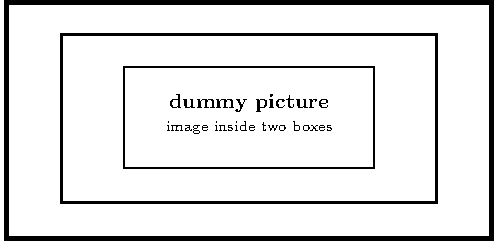
\includegraphics[width=.55\linewidth]{figures/dummy}\quad

\includegraphics[scale=.3]{figures/dummy.png}
\caption{Pictures: a PDF page scaled to a width, and a PNG image scaled by a
factor.}\label{fig:dummy}
\end{figure}

In pdfLaTeX the command runs four packages of macros: keyval parses the options,
graphics searches for the file under each known extension, graphicx turns the options
into a requested size, and the pdfTeX driver asks the engine to read the file with
\texttt{pdfximage}, measures the image in a box, writes its size back as text in big
points and reads that text again. The scale factors are found by a loop of doublings and
divisions written in macros, and every step expands tokens and makes assignments.

RushTeX runs one Rust function for the same work, with the same arithmetic: the size
is read back through big points, the factors come from the same doublings and
divisions in \TeX's integer units, and a factor times a length is rounded as \TeX{}
rounds it. The function builds the boxes the macros build, three nested boxes with the
image between a save and a restore of the graphics state and a matrix that scales it,
none at scale one. Only the file's header is read when the picture is placed; a PNG is
decoded and a PDF page copied when the document is written, once per file however
often it is shown. Loading graphicx also sets the PDF page to the paper size, as the
pdfTeX driver does, so this document's pages are letter size.

\section{Mathematics}\label{sec:math}

\subsection{How a formula is set}

Mathematics is set by the rules of Appendix~G of \textit{The \TeX book}~\cite{knuth86}.
A formula is first read into a list of \emph{noads}: an ordinary symbol, an operator, a
binary operation, a relation, an opening or closing delimiter, a fraction, a radical.
The rules then give every noad a style, a size and a position from parameters stored in
the math fonts, and insert the spaces between neighbours from a table indexed by their
classes: a thin space after an operator, a medium one around a binary operation, a
thick one around a relation. There are four styles, display, text, script and
scriptscript, and each fraction or index moves its contents one style smaller.

pdfLaTeX expands the kernel's math macros into these primitives, and runs the rules.
RushTeX ports the rules as they are and never adjusts a formula by hand; what changes is
only that the math commands are Rust functions and the symbol tables, generated from
the kernel and the packages at build time, are arrays.

\subsection{Inline formulae}

Inline formulae are written between dollar signs: $\frac{a+b}{c-d}$ is a fraction,
$\sqrt{x^2+1}$ a square root, and $x^{2}$, $a_{i}$ and $x_{i}^{2}$ show superscripts and
subscripts alone and together. Greek letters are typed by name, so $\alpha$, $\beta$,
$\gamma$ and the capital $\Gamma$ are available. Relations and operations come from
the symbol fonts: $a \leq b$, $x \neq y$, $\pm 1$, $u \cdot v$, $A \times B$, $A
\subseteq B \cup C$, $x \in A \cap B$, $\emptyset$, $p \Rightarrow q$, $p
\Leftrightarrow q$, $\forall x\, \exists y$, $\partial f$, $\nabla f$ and $x \mapsto
x^2$.

The sum $\sum_{k=1}^{n} k$ and the integral $\int_0^1 x\,dx$ set their limits beside
them in running text, as does $\lim_{n\to\infty} \frac{1}{n} = 0$. Named functions are
upright: $\sin x$, $\cos x$, $\exp x$, $\log x$, $\det A$, $\ker f$, $\max_i a_i$,
$\min_j b_j$, $\sup S$ and $\inf S$.

The set of real numbers is $\mathbb{R}$, and a bound is written $f(n) \in
\mathcal{O}(n^2)$. A vector is bold, as $\mathbf{v}$, with length $\|\mathbf{v}\|$, a
differential upright, as $\mathrm{d}x$, and a Lie algebra in Fraktur, as
$\mathfrak{g}$. Delimiters grow with what they enclose: $\left( \frac{x}{y} \right)$,
$\left[ \frac{x}{y} \right]$, $\left| \frac{x}{y} \right|$ and $\left\langle x
\right\rangle$, while $\lfloor x \rfloor$ and $\lceil x \rceil$ keep their size. The
letters of a formula stay in Computer Modern while the text is in Times, because
\LaTeX{} chooses the math fonts separately from the text family.

\subsection{Displays and equations}

Displayed formulae are centred on their own line in the display style, with larger
operators and fractions. The sum of the first $n$ integers is
\[
  \sum_{k=1}^{n} k = \frac{n(n+1)}{2}
\]
and the limits of the sum now sit above and below it. Inline formulae use the text
style, which keeps the lines of a paragraph at an even height.

Numbered equations carry labels that the text refers to. The Gaussian integral and the
quadratic formula are the next two equations.

\begin{equation}\label{eq:gauss}
  \int_{-\infty}^{\infty} e^{-x^{2}}\,dx = \sqrt{\pi}
\end{equation}

\begin{equation}\label{eq:quadratic}
  x = \frac{-b \pm \sqrt{b^{2}-4ac}}{2a}
\end{equation}

Equation~\ref{eq:gauss} gives the Gaussian integral, and Equation~\ref{eq:quadratic} the
roots of a quadratic with real coefficients $a$, $b$ and $c$, where $a \neq 0$. A
display may hold a product with a sized delimiter:
\[
  \prod_{i=1}^{m} \left( 1 + \frac{1}{i^{2}} \right) \leq e^{\pi^{2}/6}
\]

\subsection{Displayed derivations}

A derivation is a chain of displays, with the text between them giving the reason for
each step. The square of a binomial expands as
\[
  (a+b)^{2} = a^{2} + 2ab + b^{2}
\]

Applying such expansions to the terms of a sum gives a closed form for the sum of the
squares of the first $n$ integers:
\[
  \sum_{k=1}^{n} k^{2} = \frac{n(n+1)(2n+1)}{6}
\]

The formula holds for every positive integer $n$ and can be proved by induction, since
the sum for $n+1$ is the sum for $n$ with one more term. The constant $e$ is the limit
\[
  e = \lim_{n\to\infty} \left( 1 + \frac{1}{n} \right)^{n}
\]
which the reader may compare with the bound in the product above.

\section{The amsmath package}\label{sec:amsmath}

\subsection{What amsmath changes}

amsmath is the package most mathematical papers load. It changes more than it adds:
the equation number becomes a tag set by its own macros, the size of hand-sized
delimiters follows the font, the thin space and the colon get new definitions, and
accents and dots inspect what follows them. A paper that loads it is compiled natively
only if every such change is followed exactly, so RushTeX's generator sorts each name
amsmath changes into four kinds: a definition it can carry as data, a native command
that follows amsmath once it is loaded, a change that leaves the page unchanged, and a
name that sends the document to the engine path. Section~\ref{sec:packages} describes
the generator.

\subsection{Text, operators, dots and delimiters}

Words inside formulae are set in text boxes: $f(x) = 0 \text{ for all } x \in
\mathbb{R}$, and in an index $x_{\text{max}}$ the words shrink with the index. Operator
names are upright with their own spacing, as in $\tr A$, declared in the preamble with
\texttt{DeclareMathOperator}, $\operatorname{rank} M$ and
\[
  \hat{\theta} = \operatorname*{arg\,max}_{\theta} \log L(\theta), \qquad
  \bar{x} = \frac{1}{n} \sum_{i=1}^{n} x_i ,
\]
where the starred form puts the index below the name in a display.

Dots choose their height from their neighbours: $x_1, x_2, \dots, x_n$ sit on the
baseline between commas and $x_1 + x_2 + \dots + x_n$ on the axis between plus signs.
The author may also choose: $x_1 \cdots x_n$ for centred dots, $a_1, \dotsc, a_n$ for
dots between commas and $a_1 + \dotsb + a_n$ for dots between binary operations. Wide
accents stretch over their argument, as in $\widehat{xyz}$ and $\widetilde{abc}$. A map
is written $f\colon A \to B$.

Sized delimiters are written by hand when the automatic ones are too large or too
small. The four sizes, \texttt{big}, \texttt{Big}, \texttt{bigg} and \texttt{Bigg},
each come in an opening, a closing and a middle form: $\bigl( x \bigr)$, $\Bigl[ y
\Bigr]$, $\biggl\{ z \biggr\}$ and $\Biggl| w \Biggr|$. In a display:
\[
  \Big( \sum_{k} a_k \Big)^{2} \le n \sum_{k} a_k^{2} .
\]
amsmath computes their size from the height of a parenthesis in the current font, so
RushTeX's native command takes it from the same metric.

\subsection{Equations and their tags}

A numbered equation of amsmath sets its tag after the formula:
\begin{equation}\label{eq:euler}
  e^{i\pi} + 1 = 0
\end{equation}
and the \texttt{eqref} command prints the reference with its parentheses, so the text
reads \eqref{eq:euler}. A display may also go unnumbered with the starred form,
\begin{equation*}
  \vec{F} = m \ddot{x} ,
\end{equation*}
which is the same as the bracket form used in Section~\ref{sec:math}. An equation whose
number is suppressed with \texttt{notag} also has none:
\begin{equation}
  \exp(i\theta) = \cos\theta + i \sin\theta . \notag
\end{equation}

\subsection{Aligned equations in one pass}

Several equations aligned at their relation signs use \texttt{align}, which numbers each
row unless told otherwise:
\begin{align}
  (a+b)^{2} &= a^{2} + 2ab + b^{2} \label{eq:square} \\
  (a-b)^{2} &= a^{2} - 2ab + b^{2} \nonumber \\
  (a+b)(a-b) &= a^{2} - b^{2} \label{eq:difference}
\end{align}
so \eqref{eq:square} and \eqref{eq:difference} carry numbers and the middle row none.
The starred form numbers no row, and pairs of columns set several equations side by
side:
\begin{align*}
  x &= r\cos\theta, & y &= r\sin\theta, \\
  r^{2} &= x^{2} + y^{2}, & \tan\theta &= y/x .
\end{align*}

amsmath sets such a display twice: a first pass measures every column, row and tag, and
a second sets the rows with the space between the columns that the first pass found.
RushTeX sets it once. The number of columns is counted from the text before the display
starts, the rows record their widths as they are built, and at the end the same
arithmetic fixes the space before, between and after the columns and places each
number; the rows already built are then given those values. The second pass of amsmath
typesets every formula of the display again, the costliest work an alignment does, and
RushTeX does not do it at all.

\section{Packages and their options}\label{sec:packages}

\subsection{How a package becomes native}

A package is a file of macros, and pdfLaTeX reads and expands it in every run of every
document that loads it. RushTeX's generator, \texttt{rushtex-gen}, runs each package
once, at build time, on the engine path, and compares the state of \TeX{} before and
after: every parameter, every character and category code, and the meaning of every
command name. What the package added is sorted into tables: math symbols, operators,
delimiters, alphabets, font shapes, and macros whose text can be carried as data. A
name whose behaviour cannot be carried is recorded as blocked, and a document that uses
it goes to the engine path. The tables are checked against the package's own result
before they are written.

The gain is that loading a native package costs a table lookup, not the reading of its
file, and that every number it sets is the number the package itself would have set.

\subsection{Package options}\label{sec:options}

A package may be loaded with options, and the preamble of this document gives every
package it loads a few: \texttt{utf8} for inputenc, \texttt{psamsfonts} for amssymb,
\texttt{pdftex} and \texttt{final} for graphicx, and \texttt{centertags},
\texttt{sumlimits}, \texttt{nointlimits} and \texttt{namelimits} for amsmath. Each of
these asks for what the package would do anyway: UTF-8 is \LaTeX's own input encoding,
the PostScript versions of the AMS fonts are the fonts \TeX{} Live installs, pdfTeX is
the driver graphicx would choose, and amsmath already puts limits on sums and beside
integrals. So the page is the same, $\sum_{k=1}^{n} k$ and $\int_0^1 x\,dx$ inline as
well as
\[
  \sum_{k=1}^{n} \frac{1}{k^{2}} \le 1 + \int_{1}^{n} \frac{dx}{x^{2}} , \qquad
  \lim_{n \to \infty} a_n .
\]

RushTeX does not run a package's option code to find this out. Its generator loads each
package twice, once with the option and once without, and compares the whole state
afterwards. When nothing differs except the record of which options were given, the
option is entered in a table of options with no effect, and a document whose options
are all in that table stays on the native path. An option that does change something,
such as amsmath's \texttt{fleqn}, which moves displays to the left, or
\texttt{intlimits}, sends the document to the engine path until a native for it exists.

\subsection{Definitions in the preamble}

An author's own short commands are part of most papers. This document's preamble
defines one, \texttt{gdl}, which prints \gdl, with \texttt{newcommand}; it redefines the
roman family with \texttt{renewcommand} and declares an operator name with
\texttt{DeclareMathOperator}. A definition whose text uses only native commands is
native too: RushTeX expands it as \TeX{} would.

Such a command also matters to the pre-scan. To set forward references and the contents
in one pass, the pre-scan reads the headings and labels of the body ahead of
typesetting, following every counter the native commands step. An author's command could
step one it cannot see, so the pre-scan reads each definition of the preamble first: a
command whose text holds only commands that step no counter, as \texttt{gdl} does, is
passed by; any other stops the reading there, and a document that needs the rest of it
goes to the engine path. Every predicted number is still checked when its label is
reached, so a wrong prediction can only send the document to the engine, never print a
wrong number.

\section{Writing the PDF}\label{sec:pdf}

\subsection{Shipping a page}

When a page is complete, \TeX{} ships it out: it walks the page's boxes from the top
left, and for each glyph, rule and picture writes the PDF operators that place it,
changing the current font whenever the next glyph needs another. pdfTeX writes the
operators into a content stream for each page, compresses it, and at the end writes the
fonts, the pictures and the cross-reference table that lets a reader find each object.
RushTeX's shipping stage walks the same boxes, a word at a time, makes a font current
once per word, and writes the same operators in the same order, so that the two files
hold the same objects.

\subsection{Fonts in the file}

A PDF must carry the outline of every glyph it shows. pdfTeX reads each Type~1 font
program from \TeX{} Live, decrypts it, keeps only the glyphs the document uses, a
\emph{subset}, encrypts it again and embeds it. RushTeX carries the font programs in the
program itself, already decrypted, so it reads no font file; it cuts the subset as
pdfTeX cuts it, glyph for glyph, and gives it the same kind of six-letter tag.

\subsection{Compression}

Page contents and fonts are compressed with the deflate method~\cite{deutsch96}, which
codes repeated strings by reference and then codes the result with Huffman codes. pdfTeX
uses the zlib library, which builds a Huffman code fitted to each stream. RushTeX uses
the fixed code the method defines, which costs no work to build. Its files are therefore
a little larger, by a tenth to a fifth on the documents of
Section~\ref{sec:measurements}. A fitted code was tried; it made the files smaller than
pdfLaTeX's, but cost more than half a million instructions per page, and the fixed code
was kept.

\section{Exactness and the testing framework}\label{sec:testing}

Identical output is checked, not assumed. The testing framework, a separate Rust
program called parity-testing, compiles each document of a corpus with RushTeX and with
pdfLaTeX and compares the two files object by object: glyphs by font, character and
position, rules and paths by coordinates, links, outline entries and colours by value.
Then both files are rendered at 300 dots per inch and compared pixel for pixel, as
Section~\ref{sec:lists} quoted.

When a page drifts, the framework shows pdfTeX's own record of the boxes and glue above
the drifting line, so that the first node that differs can be traced back to the rule
that produced it. New native features are also compared at 150 and 600 dots per inch,
and box by box against the engine path, which is itself identical to pdfLaTeX on every
document of the corpus.

This document is the native path's own test. Each change to RushTeX must leave it on
the native path, box for box identical to the engine path, and pixel for pixel
identical to pdfLaTeX's final run. The corpus of 85 documents from CTAN must stay at
zero shift on the engine path at the same time.

\section{Measurements}\label{sec:measurements}

Speed is judged on documents of ten pages or more, against one run of pdfLaTeX, by
counting the instructions each program retires, a count that does not change with the
load of the machine. The benchmark also repeats a document's body one, four and ten
times and fits a straight line through the counts, which separates the fixed cost of a
run from the cost of each further page. The numbers below were measured on 25 October
2026, on an Apple M5 with \TeX{} Live 2026, running pdfLaTeX with
\texttt{-interaction=batchmode} and no latexmk.

\subsection{The benchmark documents}

Table~\ref{tab:bench} gives the instructions of one run of each program on the three
benchmark documents of Table~\ref{tab:results}. pdfLaTeX needed three runs for the final
PDF of each of them; RushTeX needed one.

\begin{table}[h]
\centering
\begin{tabular}{l c r r r}
Document & Pages & RushTeX & pdfLaTeX & Factor \\
\hline
Mathematics & 20 & 141.9M & 3240.2M & 22.8 \\
Tables & 29 & 205.9M & 3816.3M & 18.5 \\
Prose & 61 & 279.6M & 3280.7M & 11.7 \\
\end{tabular}
\caption{Instructions of one run, measured on 25 October 2026.}\label{tab:bench}
\end{table}

Over pdfLaTeX's three runs the factors are 72.6, 58.5 and 36.9. Peak memory is 11.5 to
17.3 megabytes for RushTeX against 29.1 to 30.1 for pdfLaTeX, and RushTeX's files are 1.1 to
1.2 times larger, as Section~\ref{sec:pdf} explains.

\subsection{Fixed cost and cost per page}

The fit separates the two costs. The column specification of the next table removes the
padding at both ends with an empty at-sign argument and repeats one column pattern with
a star.

\begin{center}
\begin{tabular}{@{}*{3}{c}@{}}
Repeats & Pages & RushTeX \\
1 & 61 & 279.1M \\
4 & 242 & 875.8M \\
10 & 603 & 2063.5M \\
\end{tabular}
\end{center}

The prose document's fit gives the costs of Table~\ref{tab:fit}.

\begin{table}[h]
\centering
\begin{tabular}{|l|c|r|}
\hline
\multicolumn{3}{|c|}{\bfseries Instructions of the prose document, from the fit} \\
\hline\hline
Program & Per page & Fixed \\
\cline{2-3}
RushTeX  & 3.3M & 78.6M \\
pdfLaTeX & 17.4M & 2220.2M \\
\multicolumn{2}{|l|}{Ratio per page} & 5.3 \\
\hline
\end{tabular}
\caption{Fixed and per-page cost, measured on 25 October 2026.}\label{tab:fit}
\end{table}

The fixed cost is 28 to 45 times smaller across the three documents, mostly because
RushTeX loads no format and reads no package or font file. The cost per page is 4.6 to
5.3 times smaller, so the factor falls as documents grow. The project's floor is forty
times on long documents too, which the per-page cost does not yet meet; the work
behind each page, Section~\ref{sec:work}, is where the rest must come from.

\section{Current limits}\label{sec:limits}

The native path is young, and its limits are part of an honest description.

\begin{itemize}
  \item It takes the article class without the \texttt{twocolumn}, \texttt{titlepage},
        \texttt{leqno} and \texttt{fleqn} options, and five packages.
  \item graphicx takes PDF and PNG pictures at a width, height or scale, but not
        rotated, clipped or in JPEG.
  \item amsmath's other multi-line environments (\texttt{gather}, \texttt{multline},
        \texttt{split}, \texttt{cases} and the matrices), \texttt{tag} and
        \texttt{binom} are not yet native.
  \item hyperref, theorems, BibTeX bibliographies, package options that change what a
        package does, input in characters outside ASCII and the T1 font encoding are not
        yet native.
  \item A page reference to a later page, a tabular column of fixed width, and a command
        the author defines with a text that could step a counter, such as one holding a
        heading, used in a document with a contents list or a forward reference, send the
        document to the engine path.
  \item The engine path needs an installed \TeX{} Live.
  \item The cost per page is about five times below pdfLaTeX's, short of the forty
        times the project aims for.
\end{itemize}

Most papers therefore still run on the engine path. Each limit is on the work list, in
the order of the papers it would unblock.

\section{What this document tests}\label{sec:tests}

Each section of this document exercises the constructs it describes. The list below
names them, commands without their backslash, so that a change to RushTeX that breaks
one shows which section to read.

\begin{description}
  \item[Front matter] \texttt{documentclass}, \texttt{usepackage} with options,
        \texttt{newcommand}, \texttt{renewcommand}, \texttt{DeclareMathOperator},
        \texttt{title}, \texttt{author}, \texttt{date}, \texttt{maketitle},
        \texttt{abstract}, \texttt{tableofcontents}.
  \item[Section~\ref{sec:intro}] \texttt{section}, \texttt{subsection},
        \texttt{emph}, \texttt{texttt}, \texttt{footnote}, forward \texttt{ref}.
  \item[Section~\ref{sec:work}] \texttt{enumerate} with a labelled item,
        nested \texttt{itemize}, \texttt{description}.
  \item[Section~\ref{sec:source}] the special characters with the braces in Times
        and in typewriter type, the tie, the accents and letters, quotes, dashes,
        \texttt{ldots}.
  \item[Section~\ref{sec:fonts}] every text font command and declaration, the
        two-letter forms, the ten sizes, groups, kerns and ligatures.
  \item[Section~\ref{sec:paragraphs}] the space factor, the at-sign and backslash
        space, \texttt{thinspace}, line breaks, \texttt{noindent}, \texttt{hspace},
        \texttt{vspace}, \texttt{mbox}, hyphenation, \texttt{cite}.
  \item[Section~\ref{sec:lists}] nested lists, \texttt{quote}, \texttt{quotation},
        \texttt{verse}, \texttt{center}, \texttt{flushleft}, \texttt{flushright},
        \texttt{centering}, \texttt{raggedright}, \texttt{raggedleft},
        \texttt{verbatim}.
  \item[Section~\ref{sec:refs-chapter}] \texttt{subsubsection},
        \texttt{paragraph}, \texttt{label}, \texttt{ref}, \texttt{pageref}, a
        footnote with an emphasis, \texttt{cite}.
  \item[Section~\ref{sec:floats}] \texttt{table} and \texttt{figure} at
        \texttt{h}, \texttt{t}, \texttt{b} and \texttt{htbp}, \texttt{figure*},
        \texttt{caption} short and long.
  \item[Section~\ref{sec:tables}] \texttt{tabular} with vertical rules,
        \texttt{hline}, a doubled rule, \texttt{cline}, \texttt{tabularnewline} with
        and without a length.
  \item[Section~\ref{sec:graphics}] \texttt{includegraphics} of a PDF at a width
        and a PNG at a scale.
  \item[Section~\ref{sec:math}] inline and display math, fractions, roots,
        indices, Greek letters, symbols, operators with limits, named functions,
        \texttt{mathbb}, \texttt{mathcal}, \texttt{mathbf}, \texttt{mathrm},
        \texttt{mathfrak}, \texttt{left} and \texttt{right}, \texttt{equation}.
  \item[Section~\ref{sec:amsmath}] \texttt{text}, \texttt{operatorname} and its
        starred form, accents, the dots, \texttt{colon}, \texttt{widehat},
        \texttt{widetilde}, the \texttt{big} family, \texttt{equation*},
        \texttt{notag}, \texttt{eqref}, \texttt{align}, \texttt{align*},
        \texttt{nonumber}.
  \item[Section~\ref{sec:packages}] package options with no effect; the preamble's
        \texttt{newcommand} used in the body, \texttt{renewcommand} and
        \texttt{DeclareMathOperator}.
  \item[Section~\ref{sec:measurements}] \texttt{tabular} with an at-sign argument
        and a starred pattern, \texttt{multicolumn}, a table with a caption.
  \item[Section~\ref{sec:bib}] \texttt{thebibliography} and \texttt{bibitem}.
\end{description}

\section{References}\label{sec:bib}

The algorithms of the native path are those of the standard references. The paragraph
builder is the method of Knuth and Plass~\cite{knuth81}; the page builder, the output
routine and the mathematics follow the reference manual of \TeX~\cite{knuth86} and its
program~\cite{knuth86b}; the hyphenation patterns follow Liang's thesis~\cite{liang83};
\LaTeX's commands follow its manual~\cite{lamport94} and its sources; compression
follows the deflate specification~\cite{deutsch96}. The chain of stages in
Figure~\ref{fig:pipeline} is a common design for compilers in general, as Aho and
colleagues describe~\cite{aho06}.

\begin{thebibliography}{9}
\bibitem{knuth81}
  Donald E.~Knuth and Michael F.~Plass.
  \emph{Breaking paragraphs into lines}.
  Software: Practice and Experience, 11(11), 1981.

\bibitem{knuth86}
  Donald E.~Knuth.
  \emph{The \TeX book}.
  Addison-Wesley, 1986.

\bibitem{knuth86b}
  Donald E.~Knuth.
  \emph{\TeX: The Program}.
  Addison-Wesley, 1986.

\bibitem{liang83}
  Franklin M.~Liang.
  \emph{Word Hy-phen-a-tion by Com-put-er}.
  PhD thesis, Stanford University, 1983.

\bibitem{lamport94}
  Leslie Lamport.
  \emph{\LaTeX: A Document Preparation System}.
  Addison-Wesley, second edition, 1994.

\bibitem{deutsch96}
  L.~Peter Deutsch.
  \emph{DEFLATE Compressed Data Format Specification version 1.3}.
  RFC 1951, 1996.

\bibitem{aho06}
  Alfred V.~Aho, Monica S.~Lam, Ravi Sethi and Jeffrey D.~Ullman.
  \emph{Compilers: Principles, Techniques, and Tools}.
  Addison-Wesley, second edition, 2006.
\end{thebibliography}

\end{document}
